\section{Simulation results}
\label{sec:ucbf-perf}
This section presents results of the simulation experiments evaluating
the performance of the UC MVDR ABF compared to the SMI MVDR and the DL
MVDR ABFs. All ABFs are implemented using $N = 11$ and $N = 51$
element ULAs and steered to the broadside look direction($\ulook =
0$). The experiments assume a passive sonar environment where the ABFs
often operate with barely sufficient snapshots $L = N + 1$ and two
snapshots per sensor $L = 2N$ is considered a snapshot rich scenario
\cite{cox2002adaptive,baggeroer1999passive}. The simulated snapshot
consists of a single loud interferer present at $\uinter = 3/N$ and a
unit power white background noise. For such measurement scenario, the
ABF output power $\pout$ is a sum of interferer contribution $\pinter$
and noise contribution $\pnoise$ as discussed in
\sect{}\ref{sec:output-power}. In the sequel, the two components of
the output power are referred to as the interferer output power
($\pinter$) and white noise output power
($\pnoise$). \sect{}\ref{sec:ucmvdr-interf-outp-result} compares the
interferer output power of the ABFs and
\sect{}\ref{sec:ucmvdr-wng-result} compares the WNGs of the
ABFs. Since the white noise output power is determined by the WNG, it
is sufficient to compare the WNGs of the ABFs. All the results are
averaged from a 3000 trial Monte Carlo experiment.

% The ABF output power is computed
% as $\pout = \wthat\herm \Cov \wthat$ where $\wthat$ is the ABF weight
% vector. Using the definition of the ECM for the single interferer case
% the output power is
% $\pout = \cov_I^2|\wthat\herm \rep_I|^2 + \cov_w^2||\wthat||^2 =
% \cov_I^2 \notchdepth + \cov_w^2 {\rm WNG}\inv = \pinter + \pnoise$.
% The total output power is the sum of interferer contribution
% ($\pinter$) and the white noise contribution ($\pnoise$).

%%% TODO
% JRB Comments
% Explain steps in order: first run UC MVDR trials, compute average WNG, then iterate estimating DL level for DL MVDR to match WNG.  Makes it clearer why you can't necessarily predict this.  

% We need to address Mestre DL algorithm at some point.  That really is the best existing benchmark, at least until Milutin Pajovic's papers are published.   

To ensure a fair comparison between the UC MVDR ABF and the DL MVDR
ABF, the DL level ($\dl$) can be chosen to match either the average
WNGs or the average notch depths (ND) between the two ABFs. In the
experiments, the DL level is chosen to match the average WNG between
the UC MVDR and the DL MVDR ABF. In order to determine the DL level,
the experiments first implement the UC MVDR for all trials and compute
the average WNG of the UC MVDR ABF. The DL level is then estimated
iteratively to match the average WNG between the UC MVDR and DL MVDR
ABFs.


\subsection{Interferer output power}
\label{sec:ucmvdr-interf-outp-result}
\figurename{}~\ref{fig:ecdf-plots} shows the empirical cumulative
distribution function (ECDF) of the interferer output power
($\pinter$) for the UC MVDR ABF compared to the SMI MVDR and DL MVDR
ABFs. The upper two panels show the ECDF graphs for the $N = 11$
sensor ULA and the lower two panels show the ECDF graphs for the $N =
51$ sensor ULA. The left two panels show the limited snapshot cases
where $L = N + 1$ and the right two panels show the snapshot rich case
where $L = 2N$. For all ULA sizes and snapshot cases, the sensor level
INR was set at $40$ dB. The dashed vertical line represents the
ensemble interferer output power $\pinter$ obtained from the MVDR
beamformer implemented using the ECM. The interferer output power
$\pinter$ corresponding to the ECDF equal to $0.5$ defines the median
value. The closer the median of the interferer output power $\pinter$
of the ABFs is to the dashed vertical line, higher the better the
probability of producing output comparable to the ensemble case. For
all four cases examined, the DL level for the DL MVDR ABF is chosen to
match the average WNGs as described earlier.

Over the observed interferer output power range in
\figurename{}~\ref{fig:ecdf-plots}, the UC MVDR ABF exhibits
higher probability of achieving lower interferer output power
$\pinter$ compared
against both SMI MVDR and DL MVDR ABFs. For instance in
\figurename{}~\ref{fig:ecdf_N11L12INR40} the median output power of UC
MVDR was approximately 20 times lower than SMI MVDR and 10 times lower
than DL MVDR ABF. The DL MVDR has improved interferer
suppression over SMI MVDR as expected, but UC MVDR has improved
performance compared to both SMI MVDR and DL MVDR ABFs.

\begin{figure}[!hp]
  \centering
  \subfloat[N = 11, L = 12]{\includegraphics[width=3in]{mvdr_smi_zfc_dl_Po_ecdf_N11L12_INR40}%
    \label{fig:ecdf_N11L12INR40}}
  \subfloat[N = 11, L = 22]{\includegraphics[width=3in]{mvdr_smi_zfc_dl_Po_ecdf_N11L22_INR40}%
    \label{fig:ecdf_N11L22INR40}}\\
  \vfill
  \subfloat[N = 51, L = 52]{\includegraphics[width=3in]{mvdr_smi_zfc_dl_Po_ecdf_N51L52_INR40}%
    \label{fig:ecdf_N51L52INR40}}
  \subfloat[N = 51, L = 102]{\includegraphics[width=3in]{mvdr_smi_zfc_dl_Po_ecdf_N51L102_INR40}%
    \label{fig:ecdf_N51L102INR40}}
  \caption[ECDF of the interferer contributed output power $\pinter$
  for the SMI MVDR, the DL MVDR and the UC MVDR ABF.]{ECDF of the
    interferer contributed output power $\pinter$ for the SMI MVDR,
    the DL MVDR and the UC MVDR ABF. The ABFs use $N = 11$ element ULA
    in the top panel and $N = 51$ element ULAs in the bottom
    panel. The left panels shows the snapshot deficient case
    ($L = N + 1$) and the right panels shows the snapshot rich case
    ($L = 2N$). In each panel the dashed vertical line denotes the
    interferer contributed output power for the ensemble MVDR ABF. In
    all cases, the UC MVDR ABF suppresses the interferer better
    compared to the SMI MVDR and DL MVDR ABFs.}
  \label{fig:ecdf-plots}
\end{figure}

\figurename{}~\ref{fig:pout-mean-var-plots} compares the squared mean
(solid) and variance (dashed) of interferer output power $\pinter$ for
UC MVDR and SMI MVDR ABFs over a range of INR values from 0 dB to 40
dB. The interferer output power $\pinter$ of the UC MVDR ABF has lower
mean and variance compared to the interferer output power $\pinter$ of
the SMI MVDR ABF. The reduced mean interferer output power $\pinter$
using UC MVDR supports the earlier conclusion that UC MVDR ABF
provides improved interferer suppression. The reduced variance on
interferer output power suggests the UC MVDR ABF should achieve better
detection performance as well.

\begin{figure*}[!hp]
  \centering
  \subfloat[L = 12 snapshots]
{\includegraphics[width=4in]{mvdr_smi_zfc_Po_meansq_var_N11_L12}%
    \label{fig:mpout_N11L12}}  \hfill
  \subfloat[L = 22 snapshots]
{\includegraphics[width=4in]{mvdr_smi_zfc_Po_meansq_var_N11_L22}%
    \label{fig:mpout_N11L22}}
  \caption[Dual y-axis plot of mean and variance of interferer output power $\pinter$ for the SMI MVDR (blue) and the UC MVDR ABF (magenta).]{Dual y-axis plot of mean and variance of interferer output power $\pinter$ for the SMI MVDR (blue) and the UC MVDR ABF (magenta). Both ABFs are implement using $N = 11$ element ULA and SCM computed from $L = 12$ snapshots in top panel and $L = 22$ snapshots in bottom panel. The UC MVDR ABF yields interferer contributed output power with lower mean and variance compared to the SMI MVDR ABF.}
  \label{fig:pout-mean-var-plots}
\end{figure*}

\subsection{White noise gain}
\label{sec:ucmvdr-wng-result}
\figurename{}~\ref{fig:wng} compares the WNG of the UC MVDR and the
SMI MVDR ABF implemented using $N = 11$ sensor ULA and $L = 12$
snapshots. The maximum WNG for this experiment is $N = 11$ and
corresponds to the CBF
\cite{vtree2002oap}. \figurename{}~\ref{fig:wng-hist-plot} compares
the histograms of the WNG for the UC MVDR and SMI MVDR ABFs. The UC
MVDR ABF achieves improved WNG compared to the SMI MVDR ABF. The
dashed vertical line denotes the ensemble WNG of $10.473$. The UC MVDR
ABF has a greater probability of achieving higher WNG with an average
WNG of $5.672$ compared to an average WNG of $2.629$ using the SMI
MVDR ABF.

\figurename{}~\ref{fig:wng-scatter-plot} is a scatter plot of the WNG
for the UC MVDR and the WNG for the SMI MVDR ABF. Each point in the
scatter plots the WNG of the UC MVDR ABF against the WNG of SMI MVDR
ABF for a single realization of the ABFs in the Monte Carlo
experiment. The scatter plot shows that the UC MVDR has a higher WNG
than SMI MVDR ABF in each trial instance except for small number of
cases (bottom left corner in \figurename{}~\ref{fig:wng-scatter-plot})
where both ABFs have low WNG. Similar results were observed for the
case of $N = 51$ sensor ULA. Thus, on average the UC MVDR ABF has a
higher WNG than the SMI MVDR ABF. In addition of being able to
suppress white noise, the improved WNG implies that the UC MVDR ABF is
also less sensitive to array parameter perturbations
\cite{Gilbert1955,vtree2002oap}.

% Although a DL MVDR is able to achieve a
% specified WNG with a choice of DL level, it requires
% numerically solving for the DL level \emph{a priori} where as UC MVDR improves the
% WNG devoid of such \emph{a priori} requirements.

\begin{figure}[!hp]
  \centering
  \subfloat[]{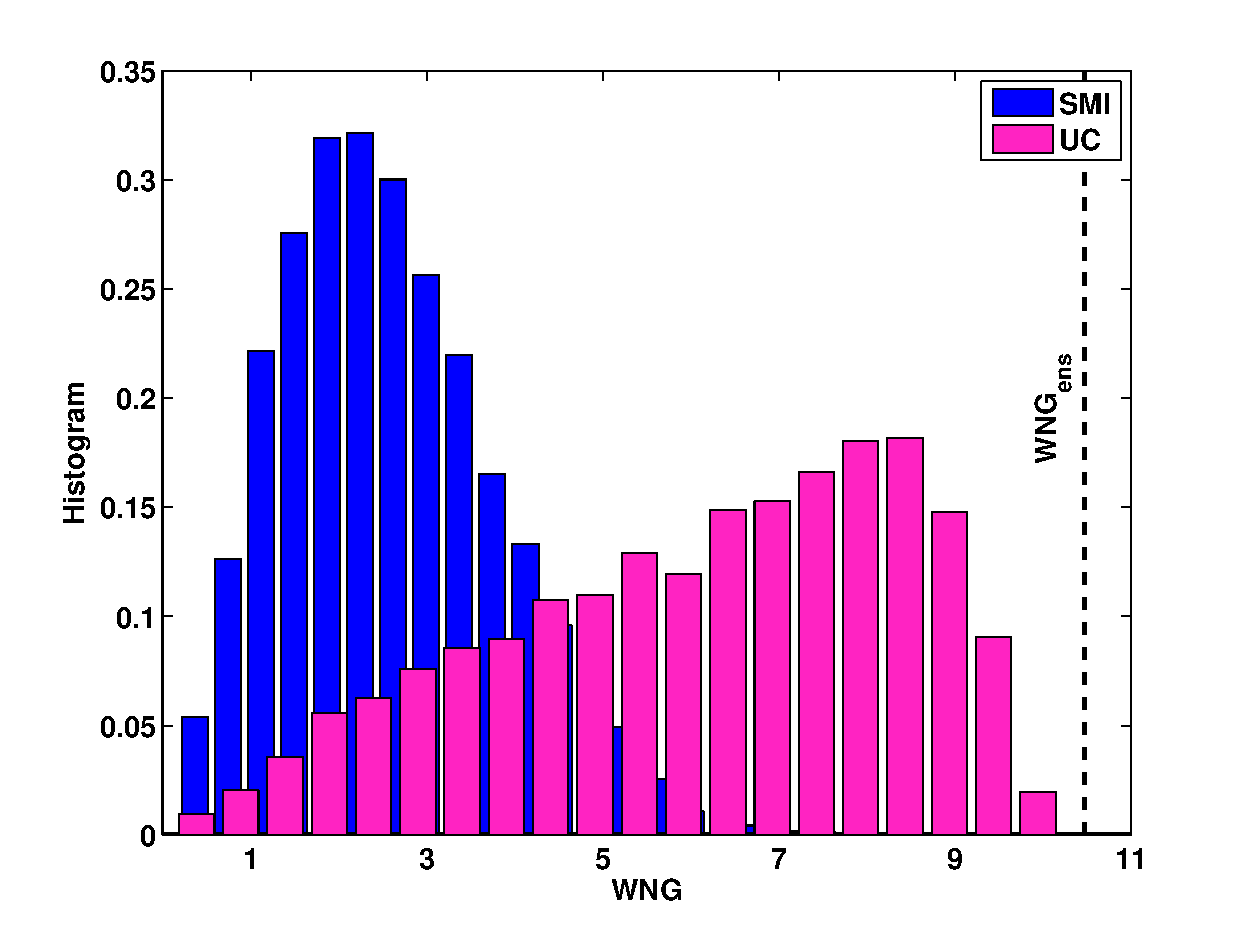
\includegraphics[width=3.5in]{mvdr_smi_zfc_WNG_hist_N11L12_INR40}
    \label{fig:wng-hist-plot}}

\subfloat[]{\includegraphics[width=3in]{mvdr_smi_zfc_WNG_scatter_N11L12_INR40}
    \label{fig:wng-scatter-plot}}
  \caption[Comparison of WNG for the UC MVDR and the SMI MVDR ABF,
    both implemented using an $N = 11$ element ULA and $L = 12$ snapshots.]{Comparison of WNG for the UC MVDR and the SMI MVDR ABF,
    both implemented using an $N = 11$ element ULA and $L = 12$
    snapshots. Top panel compares the histogram of WNGs and the lower
    panel is a scatter plot of the WNGs. On average, the UC MVDR ABF
    has higher WNG compared to the SMI MVDR ABF. }
  \label{fig:wng}
\end{figure}

\subsection{UC MVDR and DL MVDR polynomial zeros}
\label{sec:ucmvdr-dlmvdr}
The UC MVDR and the DL MVDR ABF are both derived by modifying the SMI
MVDR ABF. As described above, the UC MVDR ABF moves the sample zeros
radially back on to the unit circle. This section discusses how DL
changes the DL MVDR zeros and compares with the UC MVDR polynomial
zeros.

\figurename{}~\ref{fig:ucbf-dlsmi-pzplot} shows array polynomial zeros
a representative example of ABFs implemented using an $N = 11$ element
ULA and steered to $\ulook = 0$. A single interferer is present at
$\uinter = 3/N$ denoted by the radial dashed line. The blue squares
denote the sample zeros, the magenta circles denote the UC MVDR zeros
and the black diamonds denote the CBF zeros. Each black dot denotes a
DL MVDR zero location as the DL level changes from $-40$ dB to $40$ dB
in $4$ dB steps. When the DL level $\dl \approx 0$, the DL MVDR zeros
are essentially in sample zero locations. As the DL level increases,
the DL MVDR zeros converge towards the CBF zero locations as denoted
by the intermediate dot markers. The intermediate dot markers trace a
trajectory of DL MVDR zero locations starting from the sample zero
location to CBF zero location, as the DL level changes. A specific
trajectory is associated with each sample zero. Hence, changing the DL
level moves the DL MVDR zeros along specific trajectories. As
previously seen in \sect{}\ref{sec:diagonal-loading}, Mestre and
Lagunas present an approach to compute the optimal DL level
\cite{mestre2006finite}. The DL MVDR zeros associated with the optimal
DL level are constrained on the specific trajectories of each sample
zero, and may not be particularly close to the ensemble zero
locations. In fact, any choice of DL level always yields zeros along
the trajectories from sample zero to CBF zero
locations. Comparatively, the UC MVDR ABF approach of moving the
sample zeros radially back to the unit circle is markedly different
approach.

Moreover, one use of applying DL is to improve WNG of the ABFs
\cite{vtree2002oap}. As the DL MVDR zeros move closer to the CBF zero
locations, the WNG performance improves. However, moving zeros closer
to the CBF zero locations leads to loss of ND in the interferer
direction. Hence choosing DL level involves a trade off between loss of
interferer suppression and improved WNG. On the contrary, the unit
circle zeros of the UC MVDR create beampattern nulls which
simultaneously improve notch depth and lower sidelobes. Consequently,
the UC MVDR ABF improves both the interferer suppression and the WNG
performance as discussed in \sect{}\ref{sec:ucbf-perf}. Further, the
UC MVDR ABF does not require choosing a tuning parameter like the DL
level.

% The optimal DL level computed using Mestre and Lagunas
% \cite{mestre2006finite} approach chooses where to stop along the
% trajectory but the trajectories move
% the zeros towards the CBF zero locations instead of the ensemble zero
% locations. The DL MVDR zeros may not be particularly close to the
% ensemble zero locations.  The UC MVDR zeros do not follow the DL MVDR
% zeros trajectory and as seen above improve both WNG and interferer
% suppression.
 

% One benefit of applying DL is that it improves the WNG of the SMI MVDR
% ABF \cite{Gilbert1955}. This improvement in the WNG lowers the
% beampattern sidelobes of the ABF as mentioned earlier in
% \sect{}\ref{sec:wng}. \figurename{}~\ref{fig:ucbf-dlsmi-pzplot} shows
% that the DL MVDR ABF is able to lower the sidelobes by moving the
% polynomial zeros closer to the unit circle. As the zeros move closer
% to the unit circle, the beampattern local minimas become deeper and
% pull down the sidelobes. In contrast, the UC MVDR ABF always projects
% the SMI MVDR polynomial zeros to the unit circle. The unit circle
% zeros ensure nulls in the beampattern and also reduce sidelobes
% improving WNG. Moreover, as discussed earlier the UC MVDR ABF does not
% require an \emph{a priori} choice of a tuning parameter like the DL
% level.

\begin{figure}[!hp]
  \centering
  \includegraphics[width=\textwidth]{mvdr_smi_uc_cbf_dl_varying_pzplot}
  \caption[UC MVDR polynomial zeros compared against DL MVDR
    polynomial zeros as the DL level $\dl$ is increased from $-40$ dB to
    $40$ dB.]{UC MVDR polynomial zeros compared against DL MVDR
    polynomial zeros as the DL level $\dl$ is increased from $-40$ dB to
    $40$ dB. The DL MVDR polynomial zeros asymptotically converge to CBF polynomial zero locations as $\dl \rightarrow \infty$. }
  \label{fig:ucbf-dlsmi-pzplot}
\end{figure}

%%% Local Variables: 
%%% mode: latex
%%% TeX-master: "main"
%%% End: 
